\subsection{Ola Compiler Introduction}

The Ola-lang compiler compiles the high-level Ola contract code into the OlaAsm assembly code supported by OlaVM. 

The general pipeline process is as follows:

\begin{figure}[!htp]
    \centering
    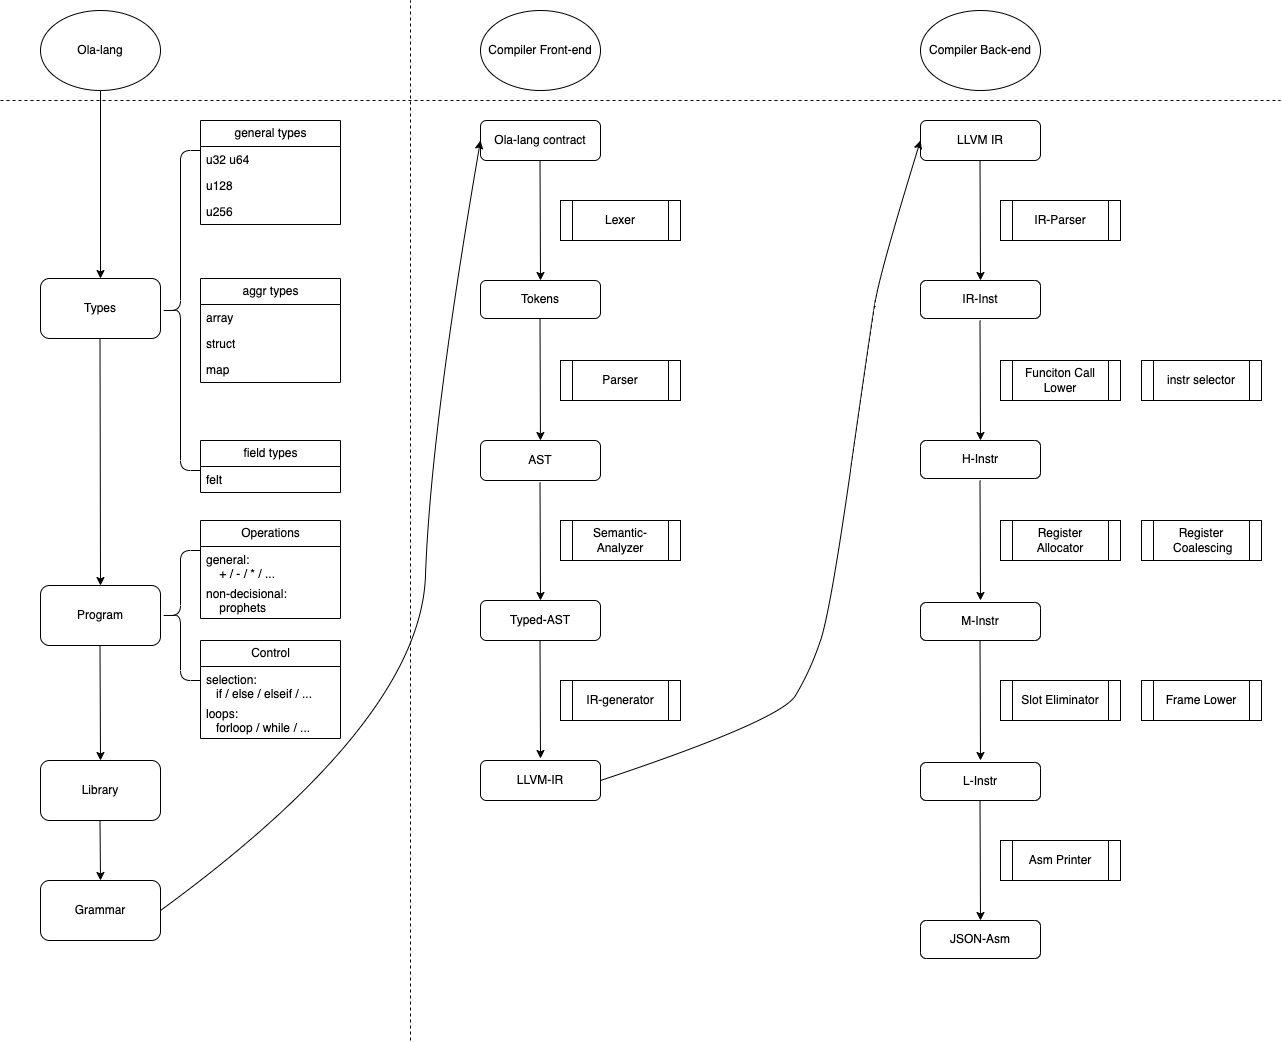
\includegraphics[width=0.8\textwidth]{ola-lang-intro.jpg}
    \caption{Ola-lang pipeline}
    \label{fig:ola-lang-intro}
\end{figure}

As can be seen from the above diagram:

The frontend of the compiler takes the high-level contract program as input and then compiles it into LLVM Intermediate Representation (IR);
and the backend of the compiler takes the LLVM IR generated by the frontend as input and then compiles it into Ola assembly code.

The assembly code is eventually assembled, linked, loaded, and executed by OlaVM through the toolchain pipeline to generate a trace.


To illustrate the compiler pipeline, the following is an example of a typical u32 type sqrt operation with instructions and Prophet two different versions to show the code generation process.

An example Ola-lang high-level language program for computing sqrt of type u32 with Prophet version is as follows:
\begin{lstlisting}[language=rust]
contract SqrtContract {

    fn main() {
       sqrt_test(4);
    }

    fn sqrt_test(u32 n) -> (u32) {
        u32 b = u32_sqrt(n);
        return b;
    }

}
\end{lstlisting}


An example ola-lang high-level language program for computing sqrt of type u32 with instructions version is as follows:
\begin{lstlisting}[language=rust]
contract SqrtContract {

    fn main() {
       sqrt_test(4);
    }

    fn sqrt_test(u32 a) -> (u32) {
        u32 result = 0;
        if (a > 3) {
            result = a;
            u32 x = a / 2 + 1;
            // assume the maximum iteration is 100
            for (u32 i = 0; i < 100; i++) {
                if (x >= result) break;
                result = x;
                x = (a / x + x) / 2;
            }
        } else if (a != 0) {
            result = 1;
        }
        return result;
    }

}
\end{lstlisting}
